\documentclass[../document]{subfiles}


\begin{document}

\section{Sprint 2}
\subsection{Introduction}
The following chapter includes all the documentation regarding the second sprint. The sprint will take place from October 6 and conclude on October 17. During this sprint, the team will make a working visualization.

During the last sprint and at the beginning of this sprint, the customer has changed their preference to the database again and now wishes to use a database designed by them. We will have to integrate this database with our system in order for our system to be satisfactory and work.

\subsection{Sprint Planning}
The total planned working hours for the second sprint is 300 hours. Of that 220 hours is to be used on implementation and 80 hours to be used on documentation, including pre-study. With 7 working members, the workload per member should be roughly 22 hours per week. We plan on spending most of this time on working with the visualiser, specifically animating it and integrating it with the new database. About 70\% of our implementation time, or more precisely 148 hours are planned for the visualiser animation and presentation. The remaining 30\% of the implementation time will be spent on database integration as well as sensor integration. We will continue to utilize pair programming, as it has proven effective in sprint 1 and there is no possibility to split the work in more than three groups. The last person will overview documentation and join any groups that need the help. 

\subsection{Sprint Goals}
The main goal of the second sprint is to create a fully functional prototype with an animated visualiser and an integrated database that can pull values from our sensors and store those values until we need to pull them in our visualiser. Our main goal can be split into five goals:
\begin{enumerate}
\item
Learn the new database received from our customer, \gls{Altran} Norge AS.
\item
Integrate the said database and data updating with the visualiser.
\item
Integrate the said database for data gathering with the central hub.
\item
Represent all types of data in the visualiser..
\item
Represent data in an interesting, animated fashion with a variable frame-rate.
\end{enumerate}

\subsection{Sprint Backlog}
Below is the sprint backlog in the form of a table, listing all of the tasks we plan to work on in this sprint. We also include the estimated working hours for each task as well as the actual amount of work spent on each task, as we complete the tasks in the sprint. The tasks also include priority, which will help the group direct their focus on the most important sub-tasks first.

\begin{table}[H]
\caption{Sprint Backlog}
\centering
\begin{tabularx}{\textwidth}{|l|X|l|l|l|}
\hline
Item
&Task
&Priority
&Estimated Hours
&Actual Hours
\\ \hline 1.1
&Integrate Altrans database with client
&H
&10
&6
\\ \hline 1.2
&Learn Altrans database
&H
&10
&6
\\ \hline 1.3
&Integrate modules from IoT-service into our project
&H
&10
&6
\\ \hline 1.4
&Open connection to db
&H
&10
&6
\\ \hline 1.5
&Query for data
&H
&15
&8
\\ \hline 1.6
&Adding new data
&H
&15
&8
\\ \hline 1.7
&Integrate Altrans database with visualiser
&H
&12
&8
\\ \hline 2.1
&Make a teardrop in JavaFX
&H
&16
&10
\\ \hline 2.2
&Create a scaling circle to represent pressure
&H
&16
&6
\\ \hline 2.3
&Create framework for circular motion
&L
&8
&4
\\ \hline 2.4
&Create framework for orbital pattern
&L
&8
&4
\\ \hline 2.5
&Create framework for moving sensors
&L
&8
&4
\\ \hline 2.6
&Make orrery
&L
&8
&6
\\ \hline 2.7
&Make animation using javafx Timeline
&L
&16
&10
\\ \hline 2.8
&Make movement gradually
&L
&16
&2
\\ \hline 2.9
&Make lighting change gradually
&L
&8
&6
\\ \hline 3.10
&Make temperature change gradually
&L
&16
&6
\\ \hline 3.11
&Make humidity change gradually
&L
&8
&6
\\ \hline 3.12
&Make pressure change gradually
&L
&10
&4
\\ \hline 
\end{tabularx}
\end{table}

\subsection{Sprint Backlog Evaluation}
The sprint plan above shows a general lack of hours. The explanation for this is two-fold.

For the visualiser module all planned features were implemented, but we overestimated the hours needed for implementation. The backlog shows 120 planned hours, with only 68 hours spent. One reason for this is that our estimate was influenced by the fact that we had estimated too few hours for the visualiser module in sprint 1, which probably caused us to add some extra hours as a buffer. Additionally, we did not take into account the knowledge we gained of JavaFX during sprint 1, which reduced the actual implementation time needed. Together, these two factors should explain the difference in hours for the visualiser module. The work hours saved were spent writing documentation.

For the database module, all planned features were implemented, except the high-priority item “Integrate \gls{Altran}'s database with client” (1.1). The backlog shows 67 planned hours, with only 48 hours spent. The estimates should be largely correct, and it is likely that the module would be finished had the planned number of work hours been invested. The imbalance between planned and spent hours is fully explained by the fact that we did not plan any overhead for the emerging high-priority tasks of writing documentation and finalizing the predelivery, which required 21.5 work hours in total of members of the database team.

\subsection{Sprint Testing}
This section covers the tests done on our system in this sprint.

\begin{table}[H]
\caption{Sprint Test 1}
\centering
\begin{tabularx}{\textwidth}{|l|X|}
\hline
Test nr
&1
\\ \hline Requirements
&4.2, 4.2.2
\\ \hline Test name
&Display the correct animation of the data in MapView
\\ \hline Environment
&Runtime
\\ \hline Description
&When the GUI starts, check if the correct data is displayed and that the animation runs smoothly when updating the database.
\\ \hline Input
&Mock up data
\\ \hline Output
&Screen holding a GUI prototype
\\ \hline Acceptance
&All of the data needs to be visible and animation needs to be correct and smooth. The animation should be spotted within 5 seconds and there should be no visual glitches.
\\ \hline Result
&When the mapview is started, there is some lag where the system mixes up the sensorIDs. However, this is a mistake with the way our database is set up and has little to do with the actual visualiser. When the database is fully integrated, we expect this bug to be solved. Furthermore, the animation is very smooth and database updates change the values and trigger animation correctly.
\\ \hline 
\end{tabularx}
\end{table}

\begin{table}[H]
\caption{Sprint Test 2}
\centering
\begin{tabularx}{\textwidth}{|l|X|}
\hline
Test nr
&2
\\ \hline Requirements
&1.1, 1.2
\\ \hline Test name
&Be able to store/change correct data
\\ \hline Environment
&Runtime
\\ \hline Description
&The database should be able to store new data or change any values in the old data at runtime, to simulate the change in sensor values.
\\ \hline Input
&Mock up data
\\ \hline Output
&Database table
\\ \hline Acceptance
&With \gls{Altran} AS database up and running, we are able to add new data and update the values of the old data at runtime.
\\ \hline Result
&Tests not conducted due to time limitations. Furthermore, \gls{Altran} AS database has very frequent downtimes, making it hard to test.
\\ \hline 
\end{tabularx}
\end{table}

\begin{table}[H]
\caption{Sprint Test 3}
\centering
\begin{tabularx}{\textwidth}{|l|X|}
\hline
Test nr
&3
\\ \hline Requirements
&4.1
\\ \hline Test name
&Send correct data to the visualiser
\\ \hline Environment
&Runtime
\\ \hline Description
&After the program has started the GUI will pull data from the database every 5 seconds. This data needs to be correctly pulled and handled.
\\ \hline Input
&Mock up data
\\ \hline Output
&Sensor data
\\ \hline Acceptance
&\gls{Altran} AS database up and running with correct data that can be manipulated and pulled when requested from the GUI. 
\\ \hline Result
&Tests not conducted due to time limitations. Furthermore, \gls{Altran} AS database has very frequent downtimes, making it hard to test.
\\ \hline 
\end{tabularx}
\end{table}

\subsection{Test Results}
In this sprint we did fewer tests than in the previous sprint. This is due to the fact that we needed to write more documentation as well as due to the fact that most of our goals revolved around implementing \gls{Altran} AS database. However, due to time constraints and limitation we had decided that testing is of less priority and have thus shortened the testing for this sprint. We are very satisfied with the animation test (the first out of the three tests here) as it produced excellent results.

\subsection{Sprint Results}
During this sprint the visualization part of our system has reached its goals, and we have completed the tasks. Changes to any data type is now reflected by an animation in the visualiser, and the animations are running in an orbit around the central hub. This is all we planned to do this sprint, and we managed to do it within the time limit of this period. 

Under is the finished mapView for this sprint. All the sensors have four elements and they circle around the central hub in different speeds.

\begin{itemize}
\item
Lighting is represented by the inner circle with the sensor name in it. It goes through a transition from white (light) to black (dark).
\item
Temperature is represented by the color of the outer circle. It goes through a transition from red (warm) to green to blue (cold).
\item
Pressure is represented by the purple balloon. It fills up for higher pressure.
\item
Humidity is represented by the blue waterdrop. It fills up for higher humidity.
\end{itemize}

\begin{figure}[H]
	\centering
	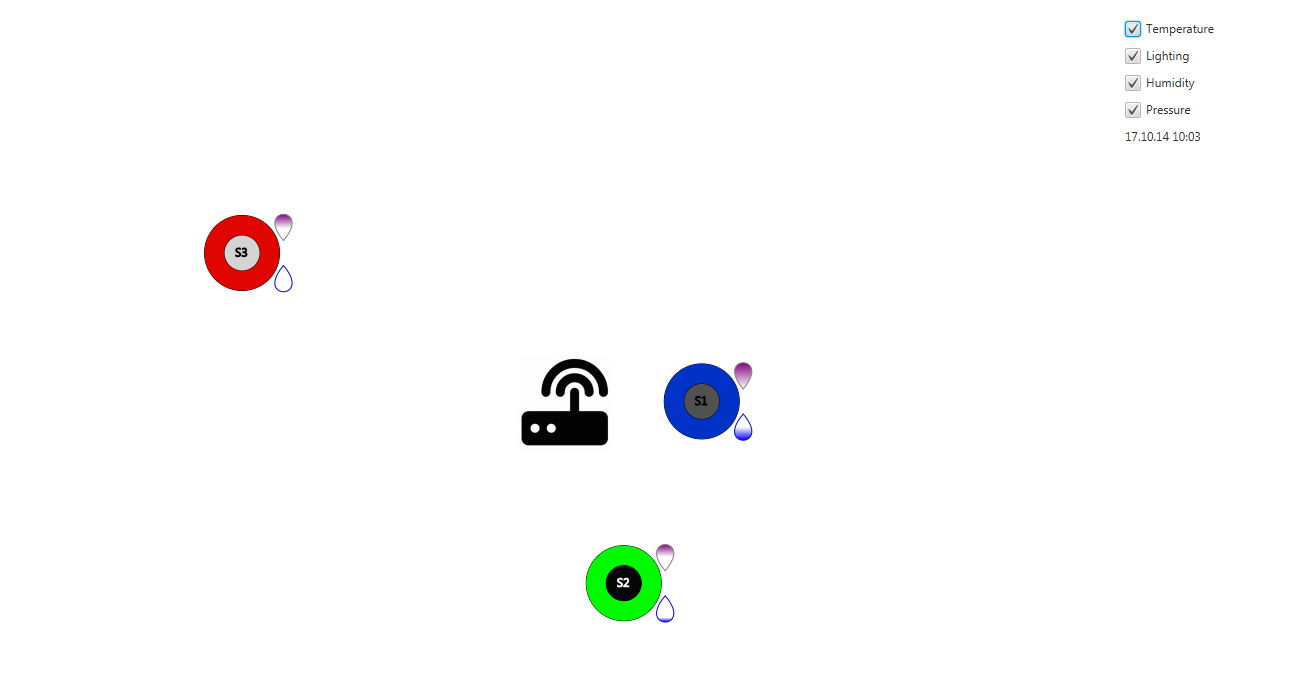
\includegraphics[width=\textwidth]{sprint_2/mapviewscreenshot.png}
	\caption{Map View}
\end{figure}

We have not yet managed to integrate the sensors into to our system. Neither have we managed to fully implement a replacement solution for the \gls{SQL}-database. The current visualiser pulls data from an \gls{SQL}-database every 5 seconds, and iterates through the data looking for changes. When the visualiser discovers a change, an animation is started that changes the appearance of the corresponding sensor. The transition is smooth, and without any glitches.

Although the new database was not integrated with the \gls{REST} of the system in this sprint, a working prototype implementation was completed. This database prototype tries to be as compliant to Altran’s database as possible. The \gls{Altran} database \gls{API} is restful, and is accessed through simple \gls{HTTP} messages. To send and receive \gls{HTTP} messages, our implementation uses the Jersey implementation of JAX-RS (\gls{Java} \gls{API} for RESTful Services).

The \gls{Altran} database also uses Apache Lucene to implement query searches against an indexed document stored in memory, sort of like a cache. This makes it possible to pull more specific sensor data with from the database. Database queries are executed by sending \gls{HTTP} GET requests with query parameters in a Lucene-specific format. When providing the visualiser with the most recent data samples, our implementation should use Lucene queries in order to limit the amount of data that has to be sent. However, this part was not implemented, as we could not manage to query for sensor samples with timestamps in a specified time interval.

Work started on integrating the new database with the visualiser, a process in which the controller class of the visualiser module went through a major refactoring. In this work it was necessary to reorganize the structure of the visualiser module to make it conformant to the style of a Maven project, a change that was largely completed.

A problem with the new database is that it is harder to insert sensor samples manually, making it somewhat less suited for testing the visualiser. This problem will be solved once our hardware person has managed to connect our sensor hardware up against a running \gls{Altran} database.

\subsection{Customer Review}
The customer is still located in Oslo, so all our meetings with the customer is done over skype. We showed him our progress and let him know our plans further. To do this we used the built in function for sharing screens. During this sprint we had a misunderstanding about when the customer meeting was supposed to be held, which led to there not being any meeting the first week of this sprint.

In an email received from the customer at the beginning of the sprint, we were informed that \gls{Altran} had a working database solution with a restful \gls{API}, and that they used it to store data collected by their own sensors. It was required that we should use the same \gls{JSON} format as \gls{Altran}:

\begin{italicquotation}
We wish for you to use the same \gls{JSON} format as us to provide interoperability. You’re free to use the code (especially for conversion) as base.
\end{italicquotation}

The customer also expressed his wishes for us to push our data to their database. This email was the basis for our decision to scrap our previous \gls{JSON}-based \gls{Cloudant} store. Instead it was decided that we should implement a new database solution during the course of the sprint, being as compliant as possible to the code of the database solution developed by \gls{Altran}. This was made a high priority task. This decision was made to minimize the risk of future change requirements. Although it was conceivable at that point to simply adapt the \gls{Cloudant} store to the new \gls{JSON} format, we would still have to get into their database \gls{API} in order to push data as requested. The difference in work hours seemed small.

In the last meeting with the customer during this sprint the customer approved our visualization, and gave us some suggestions for what we can work on in the next sprint.  

\subsection{Sprint Evaluation}
This sprint went better than sprint 1. Now we knew we would not get to integrate the hardware in time, so we focused on implementing the database and visualiser without the hardware. As we now had a better idea of what the customer actually wanted of the visualiser we could finish our suggestion. The customer was happy with our solution for visualisation, which makes this sprint a success, at least when it comes to the visualisation part. Excepting the database, we have reached all our goals, and we did not come over any major setbacks.

As for the database implementation during this sprint, until now the visualiser has used the \gls{SQL}-database from sprint 1 as a backend for testing purposes. This has worked out fine, however when the new database is ready, it will allow a much cleaner integration with both the visualiser and the hardware. Note that as a result of the database delay, two tests were not conducted.

During this sprint we have gained knowledge of Altran’s database implementation, and how it uses the Spring framework to setup a restful server for storing sensor samples, Lucene to implement queries, and an \gls{SQL}-database to store data through reboots. Another thing we have learned is how to make animations involving motions, orbital motions in particular.

\end{document}